\documentclass[conference]{IEEEtran}
\usepackage{graphicx,booktabs,amssymb,amsfonts,url}
\begin{document}
\title{Noise-Space Reinforcement Learning for Arm--Hand Coordination in a Frozen Sign Language Production Model: A Pre-registered Multi-Seed and Feasibility Study}
\author{\IEEEauthorblockN{SignSparK RL project} \and \IEEEauthorblockN{Released-checkpoint result, not a paper reproduction}}
\maketitle
\begin{abstract}We study whether reinforcement learning on the initial noise of the frozen SignSparK sign language production model can improve the coordination between generated arm and hand motion on How2Sign, which is at chance level in gloss-free generation. A 433-parameter arm-conditioned mean-shift policy (ACMS) trained with REINFORCE previously gave a small positive pre-registered result. A four-seed replication gives a pooled gain of +0.0022 [-0.0013, +0.0056] in right arm--hand coordination (registered category: seed-sensitive; I$^2$ = 0.97), about 1/23 of the registered 0.05 relevance threshold, with all preservation checks passing. A like-for-like per-clip gate (FG-1) compares learned coupling, per-clip ACMS and a bilateral variant on fresh noise. In the FG-1 fresh-noise gate: learned M-C negative (held-out $\Delta$ +0.0034); per-clip ACMS inconclusive (held-out $\Delta$ +0.1016); bilateral SC-MC positive (held-out $\Delta$ +0.0893). We conclude that the amortised RL policy yields no practically relevant improvement under the registered motion-statistic objective, while per-clip state-conditioned control is feasible. No perceptual, semantic or ASL-quality claim is made.\end{abstract}
\begin{IEEEkeywords}sign language production, reinforcement learning, rectified flow, noise-space control, pre-registration, multi-seed replication\end{IEEEkeywords}
\section{Introduction}
Sign language production (SLP) models generate signing motion from text. SignSparK [1] is a recent large rectified-flow [12] SLP model with separate body and hand generators. In its gloss-free text-to-pose regime (GF-T2P) the two hands are sampled from independent noise, and in our Stage 3 baseline the coordination between arm and hand motion in generated How2Sign [2] samples was at chance level ($\approx$ 0.02 vs $\approx$ 0.45 in the references). This project asked whether reinforcement learning (RL) on top of the \textbf{frozen} released checkpoints can reduce that deficit without degrading per-stream motion statistics.

The study was run in pre-registered, stage-gated steps. This report closes it. It presents (i) a multi-seed replication of the only training result with a positive pre-registered verdict, the arm-conditioned temporal mean-shift (ACMS) noise policy; (ii) FG-1, a like-for-like per-clip feasibility gate comparing learned M-C coupling, ACMS and a new bilateral variant under fresh noise; and (iii) a consolidated account of all executed experiments. All results are \textbf{released-checkpoint results, not a paper reproduction}, and are motion statistics only: we make no claim about perceptual naturalness, intelligibility, semantic correctness or ASL quality.

\begin{itemize}\item \textbf{C1.} A five-run replication showing that the ACMS coordination gain is \textbf{seed-sensitive} and roughly 23 times smaller than the registered 0.05 relevance threshold.\item \textbf{C2.} A fresh-noise gate (FG-1) separating in-sample from held-out controllability for three controller families on identical clips and noises.\item \textbf{C3.} A fully hashed, reproducible pipeline in which the generator, metrics, targets and thresholds were never changed after registration.\end{itemize}
\section{Problem formulation}
\subsection{Generator and action space}
SignSparK decodes a sequence of L $\leq$ 304 frames of joint-local 6D rotations (body 60, each hand 90 channels) from Gaussian noise $\varepsilon$ $\in$ $\mathbb{R}$\textasciicircum{}\{L$\times$304\} by a 10-step rectified-flow sampler conditioned on a pooled M-CLIP text embedding. The weights are frozen; the only action is the \textbf{initial noise} of a stream. One episode is one clip: the policy chooses the noise, the sampler decodes once, and a terminal reward is computed. The decision problem is therefore a contextual bandit over whole sequences (Stage 4 §4); per-frame MDPs were rejected because the generator is non-autoregressive.

\subsection{ACMS policy}
ACMS shifts the mean of the right-hand noise as a function of the generated body (arm) speed profile $\hat{s}$:

\begin{center}$\varepsilon$\_R = $\xi$ + $\mu$\_$\phi$($\hat{s}$),   $\mu$\_$\phi$($\hat{s}$) = $\beta$ $\cdot$ U $\cdot$ tanh(W $\ast$ $\hat{s}$ + c),   $\xi$ $\sim$ N(0, I)\end{center}
with rank r = 4, a 17-tap temporal kernel W, and 433 trainable parameters. Because only the mean shifts, the policy KL to the uncoupled sampler is ½$\|$$\mu$$\|$$^2$ per frame and is bounded below 1 nat/frame by construction. Training uses REINFORCE [3] with a leave-one-out baseline over G = 4 draws per clip [4], Adam (lr 0.01), gradient clipping at 1.0, and 125 updates (500 episodes) on TRAIN clips.

\subsection{Reward and constraints}
The reward is target matching on right arm--hand coordination in rotation space R (metric v1.1): r = --|coord\_ah\textasciicircum{}R -- 0.4514|, where 0.4514 is the frozen train-reference target (R0). Articulation, jerk, extreme-pose and activity constraints enter through Lagrangian dual ascent [5]; $\lambda$ remained 0 in every group of every run, so no constraint became active.

\subsection{Evaluation statistic}
The primary statistic is the paired clip-mean difference in right arm--hand coordination (R) between the trained policy (update 125) and the uncoupled sampler on dev-256 $\times$ 4 shared evaluation noises (base 40M). Joint-space (J, SMPL-X [9]) analogues are descriptive only; R and J are different metrics on the same samples and are \textbf{not} independent replications.

\section{Experimental protocol}
\subsection{Multi-seed replication}
Seeds 7001--7004 each vary three sources independently: policy initialisation (init seed = run seed), training-clip sampling (sampler seed 5000 + d) and training noise (base 50M + d$\cdot$1M). Evaluation noise is shared. The original configuration and code were reused unchanged (SHA-verified); the four runs were trained and evaluated sequentially. Training runs are the unit of inference: we report per-run estimates, a t-interval across runs, a clip bootstrap of seed-averaged per-clip $\Delta$ (evaluation-sampling uncertainty only), a hierarchical bootstrap, and heterogeneity (Cochran's Q, I$^2$, DerSimonian--Laird $\tau$$^2$ [10]). Run 7000 enters only the secondary five-run pool. The category rule (registered before the runs) is: inconclusive (validity) $\rightarrow$ negative $\rightarrow$ reproducible positive $\rightarrow$ seed-sensitive $\rightarrow$ inconclusive (precision).

\subsection{FG-1 per-clip feasibility gate}
FG-1 asks whether any controller family can raise held-out coordination on clips it was fitted to, when evaluated on fresh noise. Sixteen TRAIN clips (8 with L < 100, 8 with L $\geq$ 100; seeded selection excluding all ACMS training clips) each get 16 fitting noises (base 60M) and 16 held-out noises (base 61M). Per-clip parameters are fitted with pathwise gradients through the unrolled, checkpointed sampler (Adam lr 0.05, 30 iterations) on a chordal-speed surrogate of the coordination statistic.

\begin{itemize}\item \textbf{V0} uncoupled sampler (reference).\item \textbf{V1} learned M-C: Stiefel-SVD coupling of right-hand noise to body noise, $\kappa$ $\leq$ 0.9 (E2c (ii) family).\item \textbf{V2} per-clip ACMS (433 parameters, as in §II-B).\item \textbf{V3} bilateral SC-MC: two ACMS heads (right on right arm, left on left arm), objective = surrogates of right, left and left--right coordination (new, authorised direction).\end{itemize}
Outcome per statistic: positive if the 95\% clip CI lower bound > 0, the point estimate $\geq$ 0.05 and preservation passes; negative if the CI upper bound < 0.05; otherwise inconclusive. Operational decisions D1--D10 (e.g. a 120-min cap for V3 and 8 rows per pass) were documented before any FG-1 run and change no scientific setting.

\subsection{Safeguards}
\begin{itemize}\item SignSparK checkpoint SHA-256 verified before and after all experiments; weights-unchanged checksum in every job.\item Seed and noise-base disjointness preflight; configuration and code hashes recorded.\item Stage 4/5 artifacts snapshotted (SHA-256) and re-verified at closure; new outputs in separate directories.\item Only registered TRAIN and DEV splits opened; the How2Sign test split was never opened.\item Registered metrics, validity rules, frozen targets, rewards and thresholds unchanged.\end{itemize}
\section{Results: ACMS multi-seed replication}
All four new runs completed (500 episodes each) with weights unchanged, zero undefined statistics and zero validity flags. The uncoupled evaluation outputs were bitwise identical across runs, so every run is compared against the same baseline samples.

\begin{table*}[t]\centering\caption{Per-run ACMS results (dev-256 $\times$ 4, space R)}\footnotesize\begin{tabular}{llllllll}\toprule \textbf{Run} & \textbf{$\Delta$ coord\_ah\textasciicircum{}R [95\% clip CI]} & \textbf{single-run verdict} & \textbf{$\Delta$ dominance} & \textbf{$\Delta$ L--R} & \textbf{KL mean} & \textbf{train s} & \textbf{eval s} \\ \midrule 7000 & +0.0022 [+0.0014, +0.0031] & positive & +0.0029 & +0.0006 & 0.0037 & 284 & 1639 \\ 7001 & -0.0003 [-0.0007, +0.0001] & negative & -0.0009 & +0.0001 & 0.0026 & 283 & 1694 \\ 7002 & +0.0011 [+0.0005, +0.0016] & positive & -0.0014 & -0.0003 & 0.0029 & 282 & 1556 \\ 7003 & +0.0041 [+0.0032, +0.0052] & positive & +0.0006 & +0.0002 & 0.0035 & 273 & 1551 \\ 7004 & +0.0039 [+0.0030, +0.0049] & positive & +0.0038 & -0.0006 & 0.0088 & 273 & 1551 \\ \bottomrule\end{tabular}\end{table*}
Run-level effects range from -0.0003 (run 7001, CI includes 0, single-run verdict negative) to +0.0041. The pooled four-run mean is +0.0022 [-0.0013, +0.0056] (t-interval, SD 0.00217); the CI includes zero. The clip bootstrap +0.0022 [+0.0018, +0.0026] reflects only evaluation sampling and is therefore much narrower. Heterogeneity is high (Q = 108.0, df = 3, I$^2$ = 0.97). The registered category is \textbf{seed-sensitive}. The secondary five-run pool gives +0.0022 [-0.0001, +0.0045] (seed-sensitive).

\begin{figure*}[t]\centering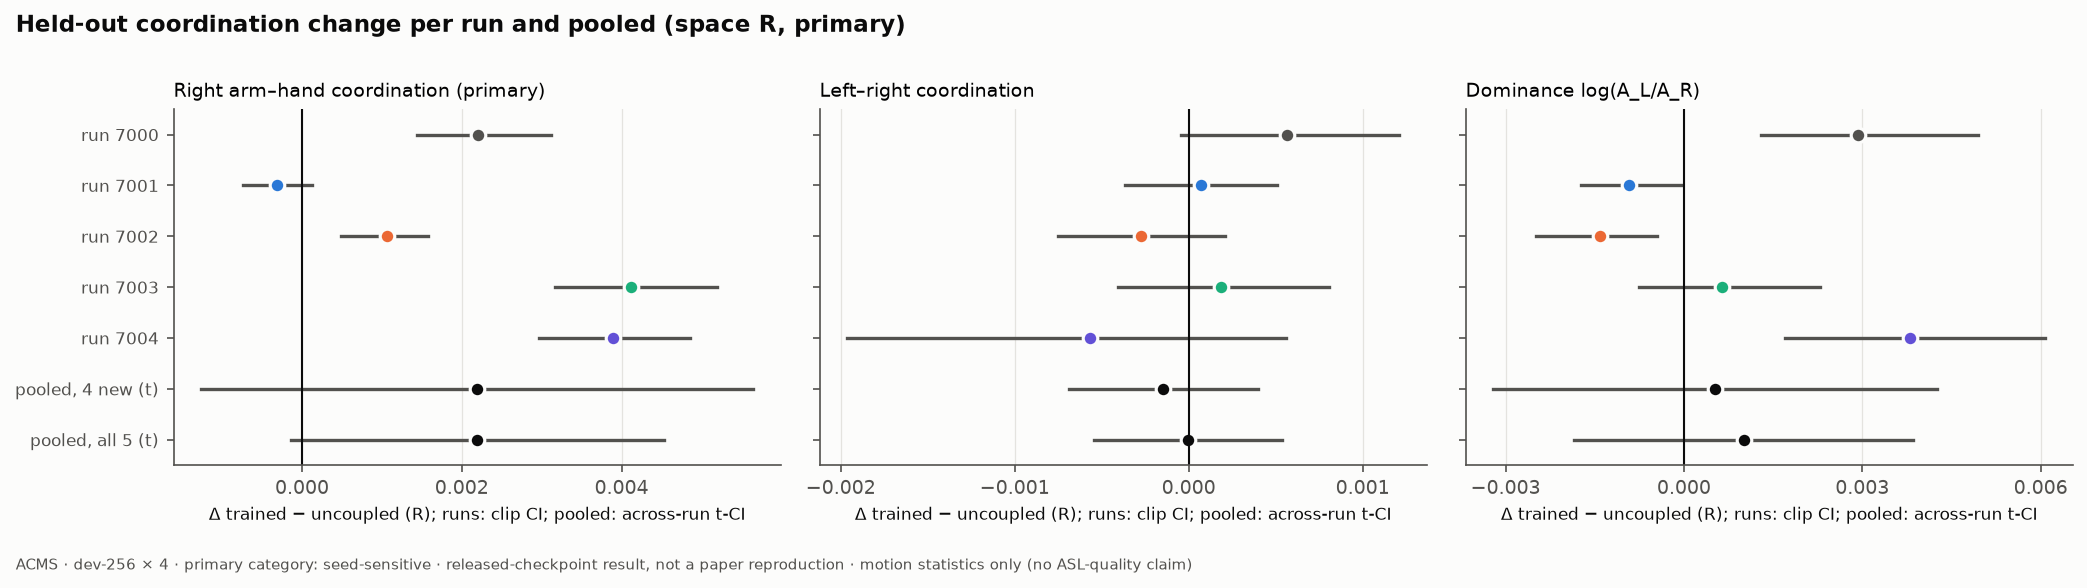
\includegraphics[width=\textwidth]{figures/f04_coordination_multiseed.png}\caption{Held-out change in right arm--hand coordination, left--right coordination and dominance per run (95\% clip CI) and pooled (t-interval across runs). Space R.}\end{figure*}
Magnitude: even the largest run closes about 1.0\% of the gap to the 0.4514 target, and no run reaches the 0.05 threshold (pooled ratio to 0.05: 0.044). Dominance and left--right coordination show no consistent direction across runs. The trained -- initial contrast (pooled +0.0020 [-0.0010, +0.0050]) and the initial -- uncoupled contrast (+0.0002 [-0.0012, +0.0015]) are reported as the ablation of training versus random initialisation.

\begin{figure}[t]\centering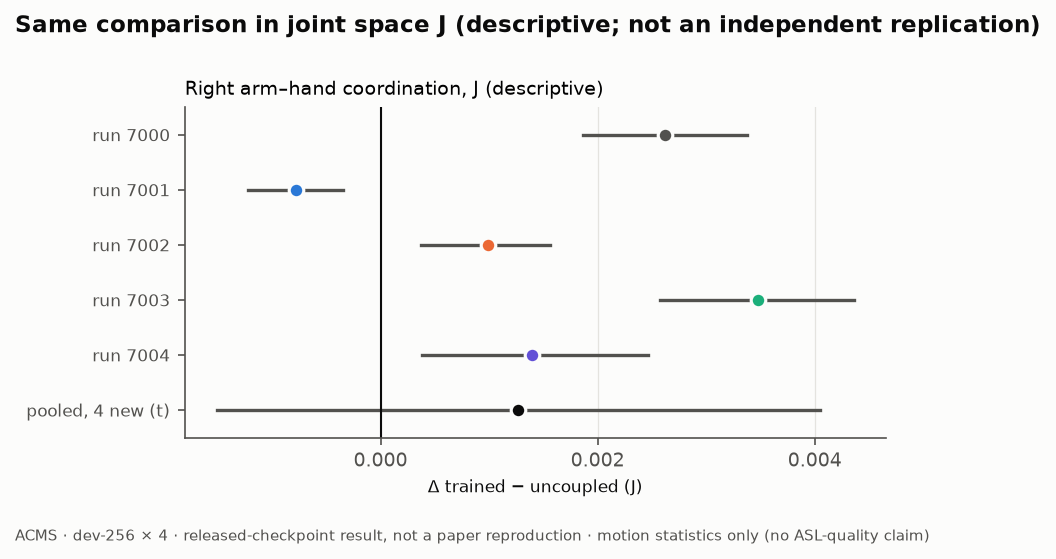
\includegraphics[width=\columnwidth]{figures/f04b_coordination_multiseed_J.png}\caption{Joint-space (J) analogues, descriptive. Same samples as Fig. 1; not an independent replication.}\end{figure}
\subsection{Preservation}
\begin{table}[t]\centering\caption{Pre-registered preservation checks (trained vs uncoupled)}\footnotesize\begin{tabular}{llll}\toprule \textbf{Check (limit)} & \textbf{Pooled mean, 4 new runs} & \textbf{Range over 5 runs} & \textbf{All pass} \\ \midrule articulation ratio (0.9--1.1) & 1.0002 & 0.9978--1.0018 & yes \\ jerk ratio ($\leq$ 1.1) & 0.9998 & 0.9967--1.0015 & yes \\ extreme-pose diff ($\leq$ 0.02) & 0.0000 & 0.0000--0.0000 & yes \\ |log activity ratio| ($\leq$ 0.223) & 0.0017 & 0.0006--0.0038 & yes \\ KL max nats/frame ($\leq$ 1) & 0.0056 & 0.0032--0.0114 & yes \\ \bottomrule\end{tabular}\end{table}
Every preservation check passes in every run, with ratios within 0.5\% of 1. Combined with a maximum KL of 0.0114 nats/frame, this shows that ACMS operates as a very small perturbation of the base sampler; the tiny effect is consistent with that.

\begin{figure*}[t]\centering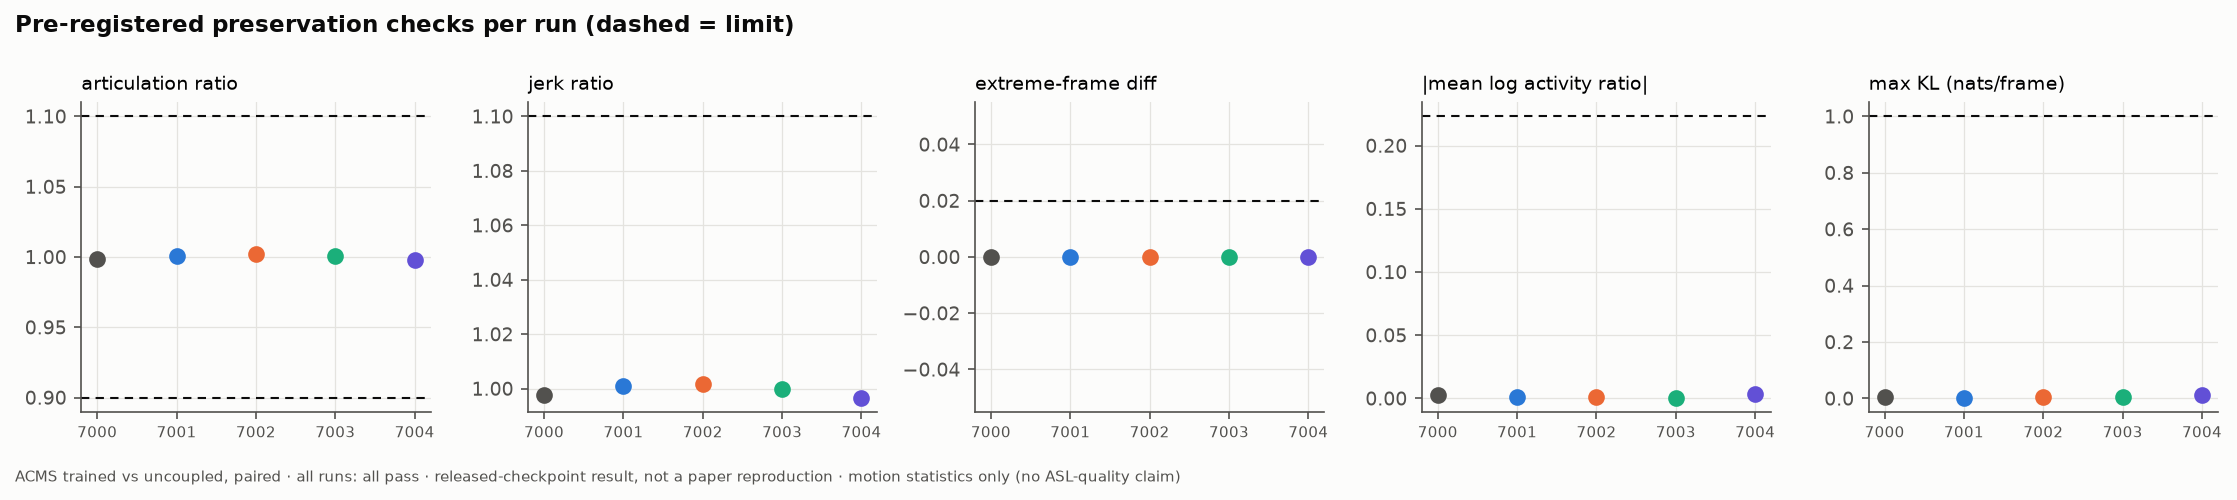
\includegraphics[width=\textwidth]{figures/f05_preservation_multiseed.png}\caption{Preservation checks per run; dashed lines are registered limits.}\end{figure*}
\subsection{Training dynamics and checkpoints}
\begin{figure*}[t]\centering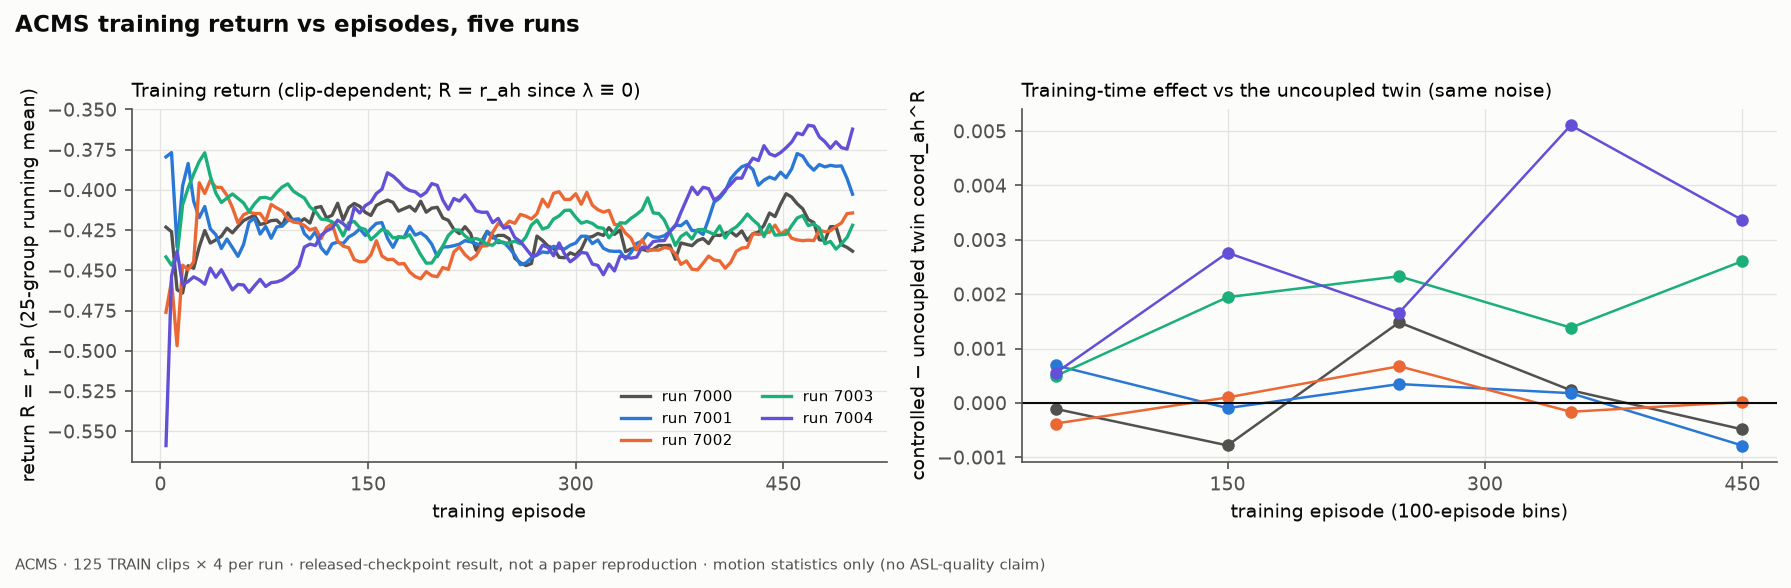
\includegraphics[width=\textwidth]{figures/f01_training_return.png}\caption{Training return (left) and training-time controlled -- twin coordination (right, 100-episode bins) for all five runs.}\end{figure*}
Pooled held-out $\Delta$ by checkpoint (4 new runs, t-intervals): update 0: +0.0002 [-0.0012, +0.0015]; update 25: +0.0006 [-0.0014, +0.0026]; update 50: +0.0008 [-0.0024, +0.0040]; update 75: +0.0011 [-0.0020, +0.0043]; update 100: +0.0019 [-0.0009, +0.0047]; update 125: +0.0022 [-0.0013, +0.0056]. Update 125 remains the primary and only pre-registered checkpoint; intermediate checkpoints were evaluated for monitoring only and none was selected.

\begin{figure*}[t]\centering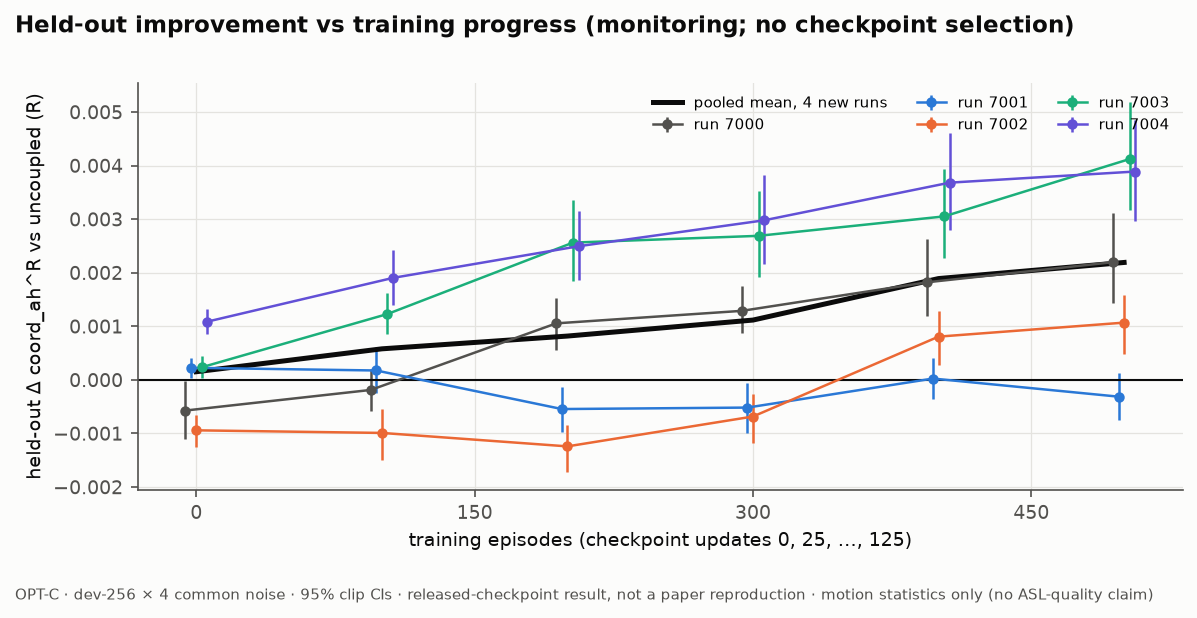
\includegraphics[width=\textwidth]{figures/f02_heldout_vs_progress.png}\caption{OPT-C: held-out $\Delta$ at updates 0--125 (monitoring only).}\end{figure*}
\begin{figure}[t]\centering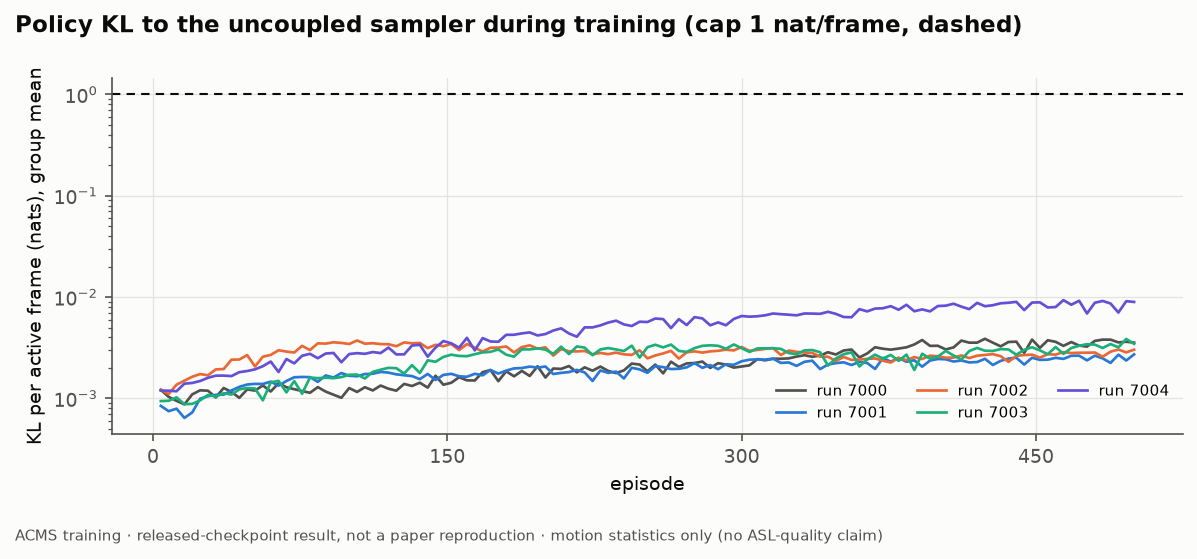
\includegraphics[width=\columnwidth]{figures/f06_kl_multiseed.png}\caption{Policy KL to the uncoupled sampler during training.}\end{figure}
\begin{figure}[t]\centering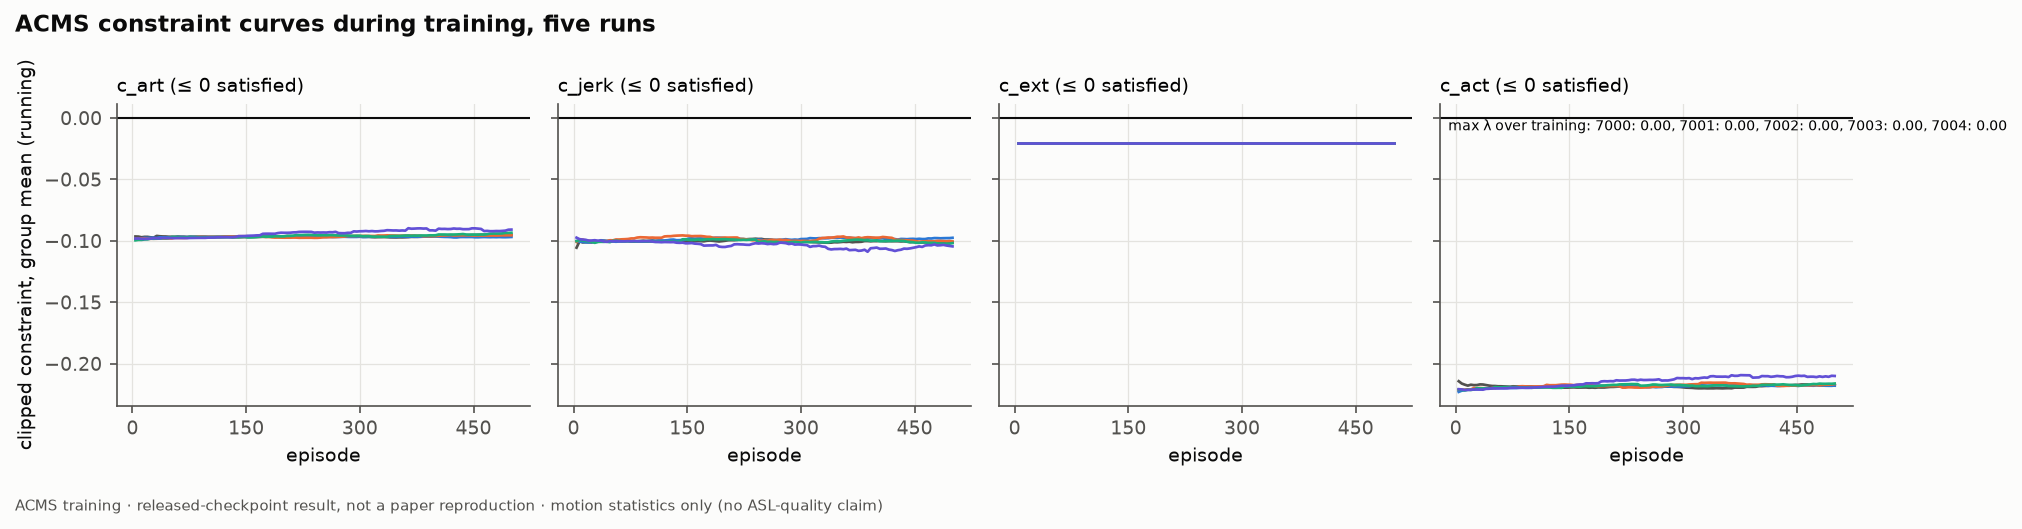
\includegraphics[width=\columnwidth]{figures/f03_training_constraints.png}\caption{Constraint values during training; $\lambda$ remained 0 throughout.}\end{figure}
\subsection{Stability}
\begin{figure*}[t]\centering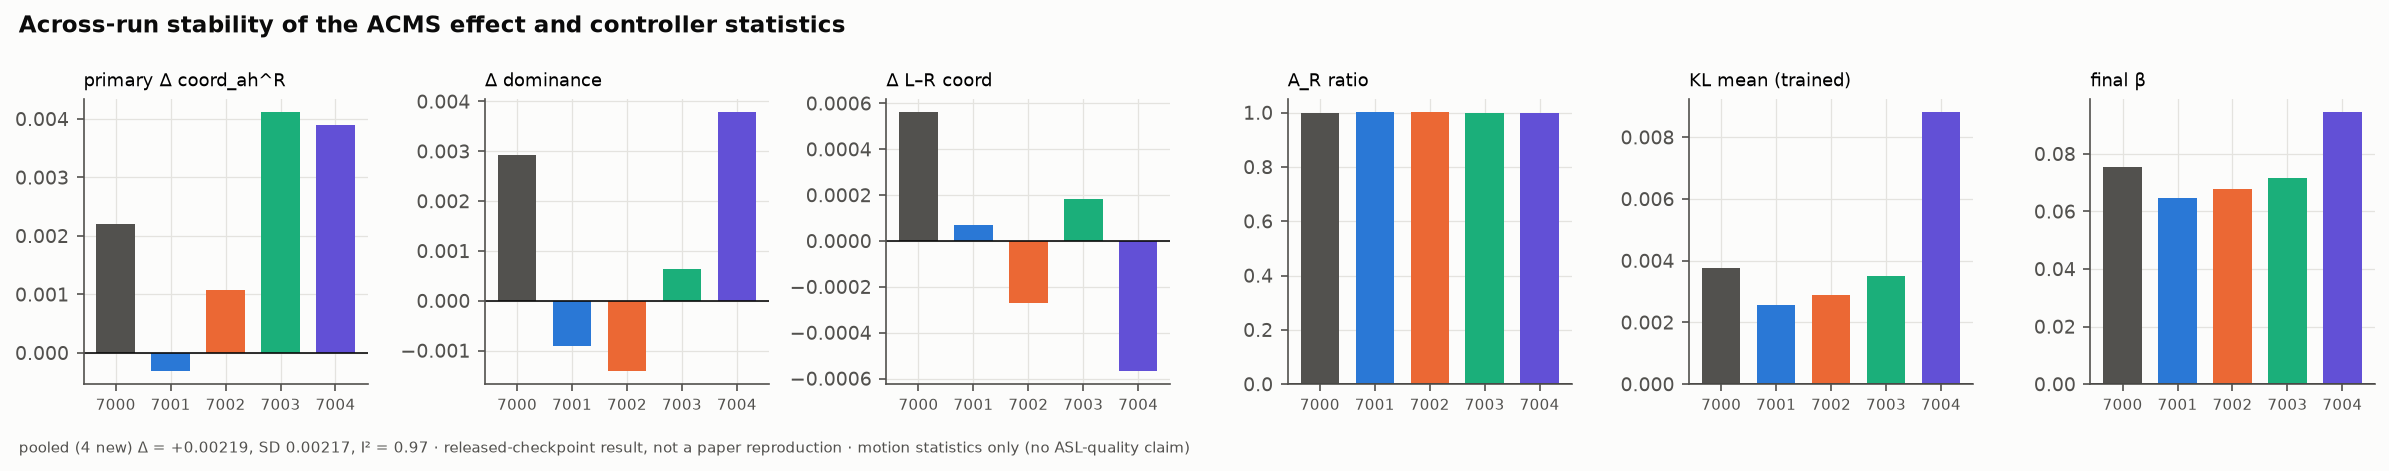
\includegraphics[width=\textwidth]{figures/f09_seed_stability.png}\caption{Across-run spread of the effect and controller statistics.}\end{figure*}
\section{Results: FG-1 feasibility gate}
The uncoupled baseline V0 has held-out right arm--hand coordination +0.062 [+0.028, +0.098] on the 16 gate clips; the best-of-16 selection context (maximum over the 16 held-out V0 draws, an oracle that a policy cannot use) is +0.401 [+0.316, +0.494]. The registered threshold for a positive outcome is a held-out gain of 0.05 with the 95\% clip CI lower bound above zero and all preservation checks passing.

\textbf{V1 (learned M-C coupling).} Held-out $\Delta$ +0.0034 [-0.0121, +0.0166] (10/16 clips positive); in-sample $\Delta$ at the last iteration +0.4938 [+0.4418, +0.5447]; generalisation gap +0.4904 [+0.4365, +0.5451]. KL max 2.98 nats/frame (right). Preservation passes. Registered outcome: \textbf{negative}.

\textbf{V2 (per-clip ACMS).} Held-out $\Delta$ +0.1016 [+0.0753, +0.1288] (15/16 clips positive); in-sample $\Delta$ at the last iteration +0.2058 [+0.1849, +0.2245]; generalisation gap +0.1042 [+0.0714, +0.1394]. KL max 0.119 nats/frame (right). Preservation fails. Registered outcome: \textbf{inconclusive}. State-shuffle ablation ($\hat{s}$ from a different noise draw), shuffled -- matched: -0.0853 [-0.1093, -0.0605].

\textbf{V3 (bilateral SC-MC).} Held-out $\Delta$ +0.0893 [+0.0703, +0.1091] (16/16 clips positive); in-sample $\Delta$ at the last iteration +0.1765 [+0.1559, +0.1983]; generalisation gap +0.0872 [+0.0645, +0.1117]. KL max 0.112 nats/frame (right). Preservation passes. Registered outcome: \textbf{positive}. Left arm--hand $\Delta$ +0.1071 [+0.0795, +0.1352] (positive); left--right $\Delta$ +0.0333 [+0.0049, +0.0594] (inconclusive); KL max left 0.126. State-shuffle ablation ($\hat{s}$ from a different noise draw), shuffled -- matched: -0.0730 [-0.0947, -0.0496].

\begin{table*}[t]\centering\caption{FG-1 per-variant results (16 TRAIN clips, held-out = 16 fresh noises per clip, space R)}\footnotesize\begin{tabular}{llllllll}\toprule \textbf{Variant} & \textbf{Params/clip} & \textbf{Held-out $\Delta$ vs V0 (R, right)} & \textbf{In-sample $\Delta$ (last iter)} & \textbf{Gap} & \textbf{KL max} & \textbf{Preserv.} & \textbf{Outcome} \\ \midrule V1 & 9060 & +0.0034 [-0.0121, +0.0166] & +0.4938 [+0.4418, +0.5447] & +0.4904 & 2.980 & pass & negative \\ V2 & 433 & +0.1016 [+0.0753, +0.1288] & +0.2058 [+0.1849, +0.2245] & +0.1042 & 0.119 & FAIL & inconclusive \\ V3 & 866 & +0.0893 [+0.0703, +0.1091] & +0.1765 [+0.1559, +0.1983] & +0.0872 & 0.112 & pass & positive \\ \bottomrule\end{tabular}\end{table*}
\begin{figure*}[t]\centering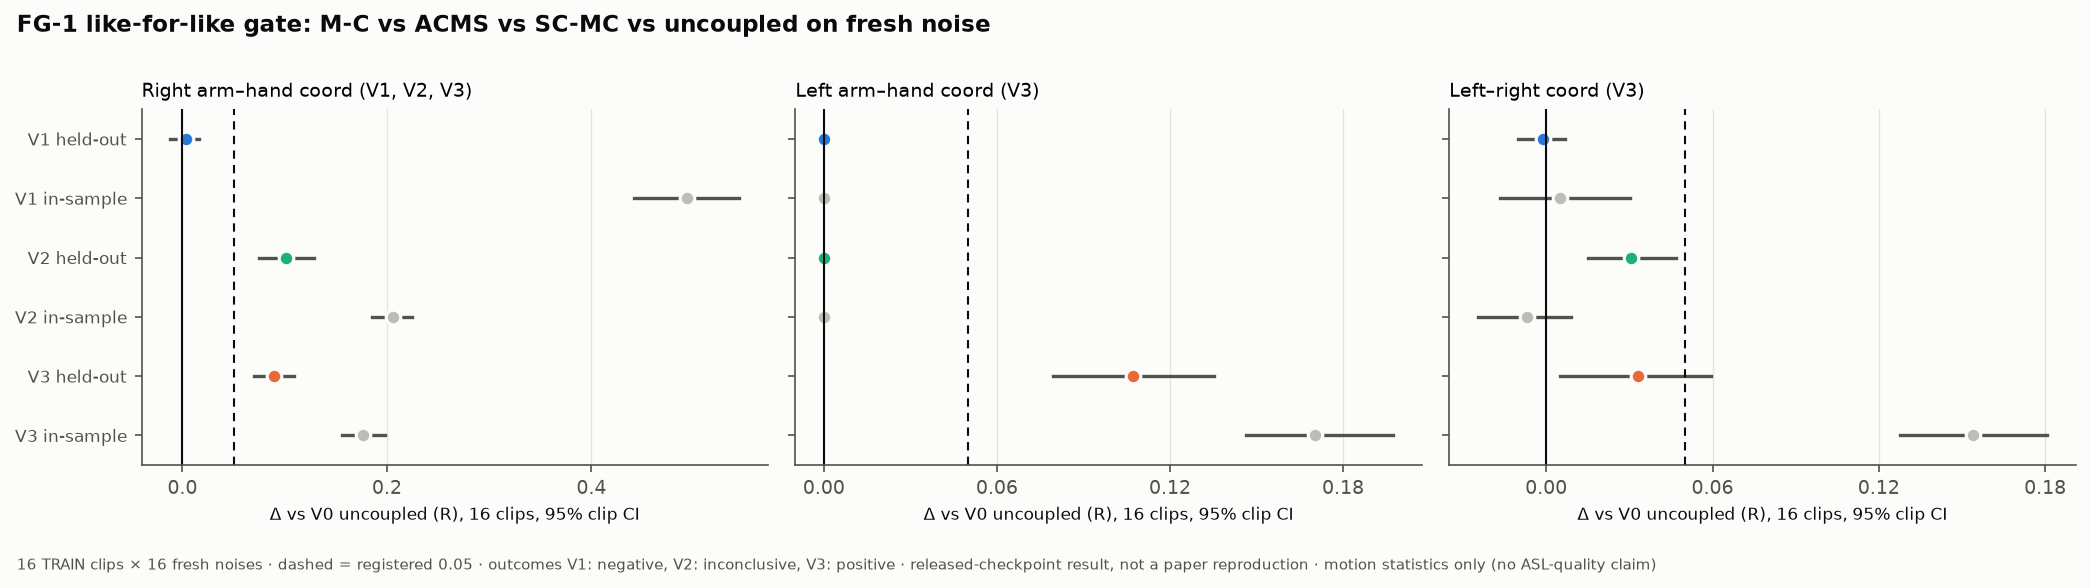
\includegraphics[width=\textwidth]{figures/f08_fg1_comparison.png}\caption{FG-1 held-out vs in-sample $\Delta$ per variant and statistic; dashed = 0.05.}\end{figure*}
\begin{figure}[t]\centering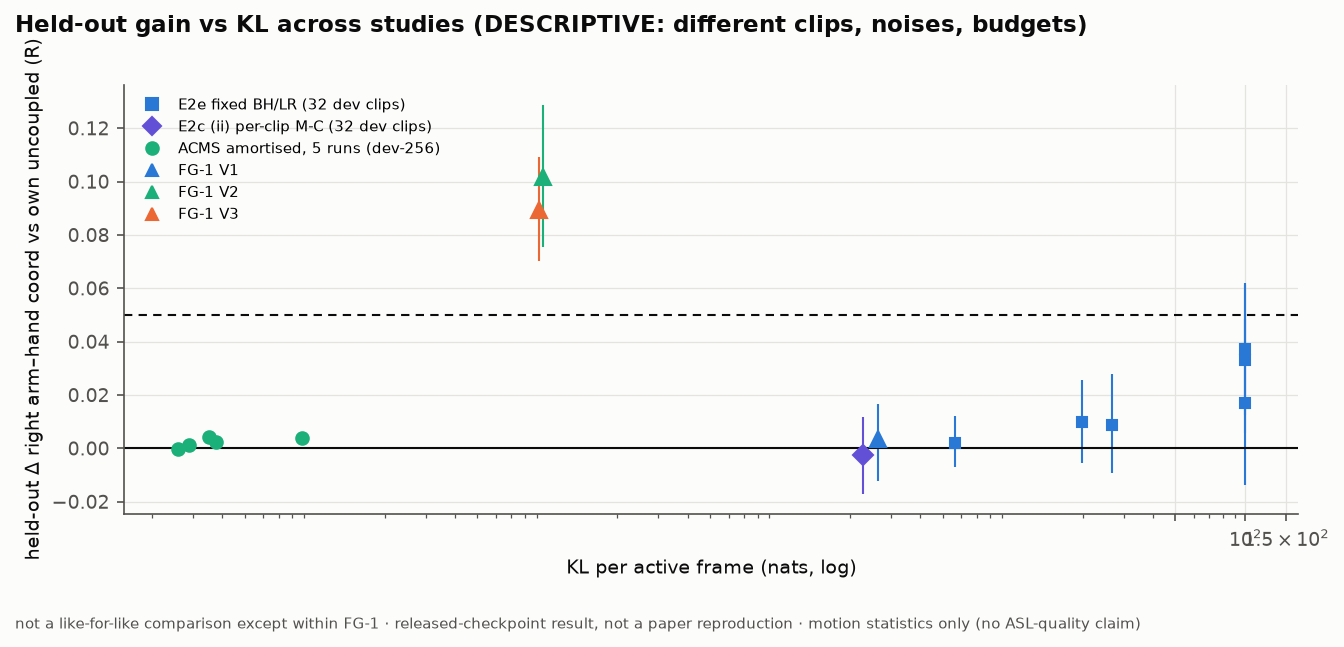
\includegraphics[width=\columnwidth]{figures/f08b_cross_study_kl.png}\caption{Held-out gain vs KL across studies. Descriptive only: studies differ in clips, noises and budgets; only FG-1 is like-for-like.}\end{figure}
\section{Generalisation, ablations and computation}
OPT-G (each run's own 125 TRAIN clips, fresh noise base 45M, four draws): pooled $\Delta$ +0.0019 [-0.0015, +0.0053] vs the dev $\Delta$ +0.0022 [-0.0013, +0.0056]; pooled train -- dev gap -0.0003 [-0.0018, +0.0011]. This compares training-distribution clips to unseen dev clips under fresh noise; it is monitoring, not a selection criterion.

\begin{figure*}[t]\centering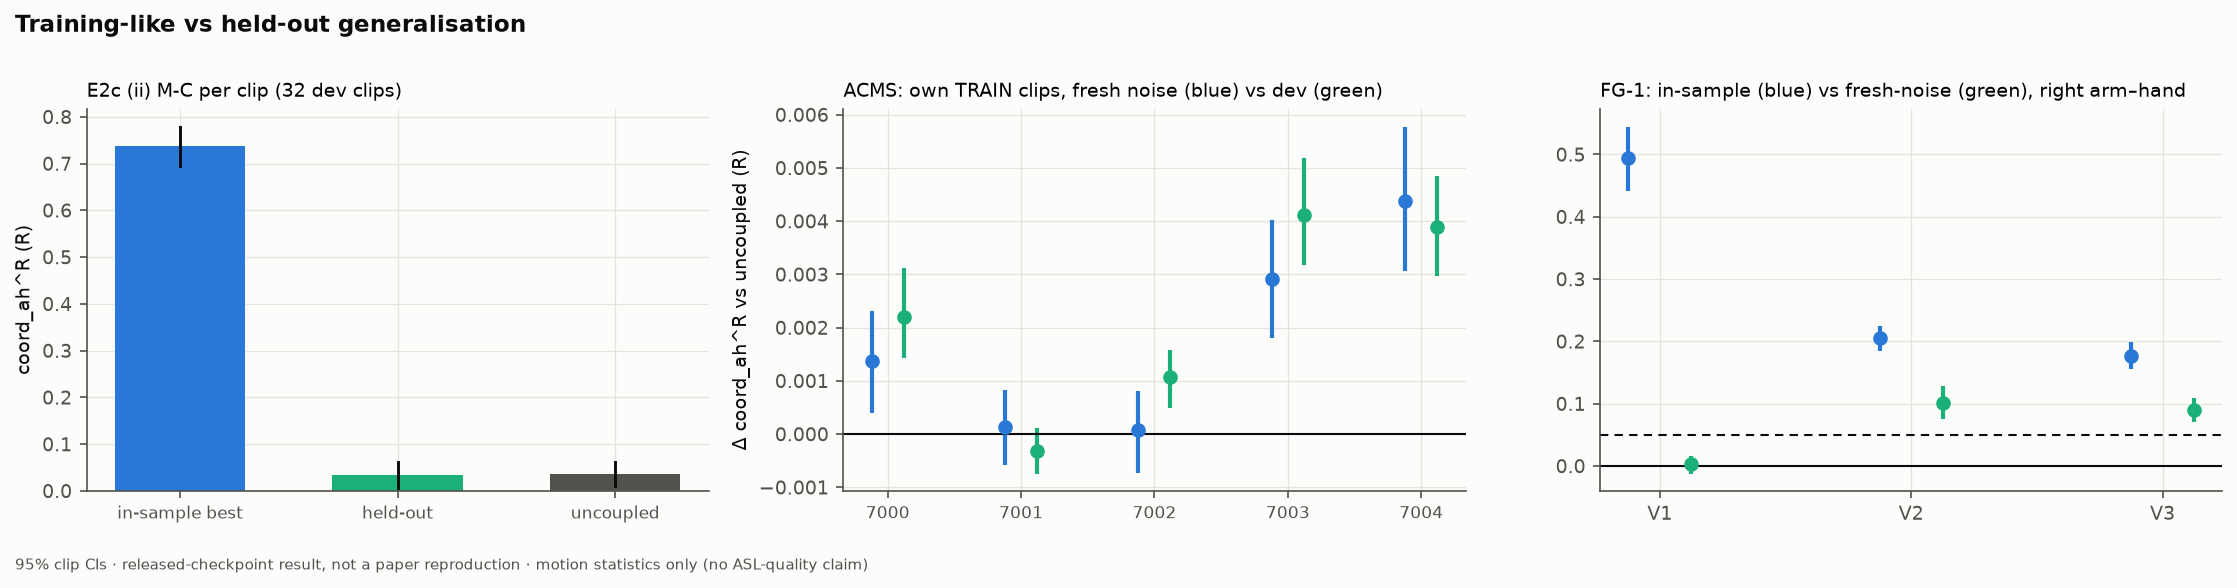
\includegraphics[width=\textwidth]{figures/f10_generalisation.png}\caption{In-sample vs held-out: E2c (ii), ACMS OPT-G vs dev, FG-1.}\end{figure*}
Ablations actually run: (a) trained vs initial policy and initial vs uncoupled (all ACMS runs); (b) FG-1 state-shuffle, replacing the conditioning signal $\hat{s}$ with that of a different noise draw (V2, V3). No other ablation was run, and none is implied.

\begin{figure*}[t]\centering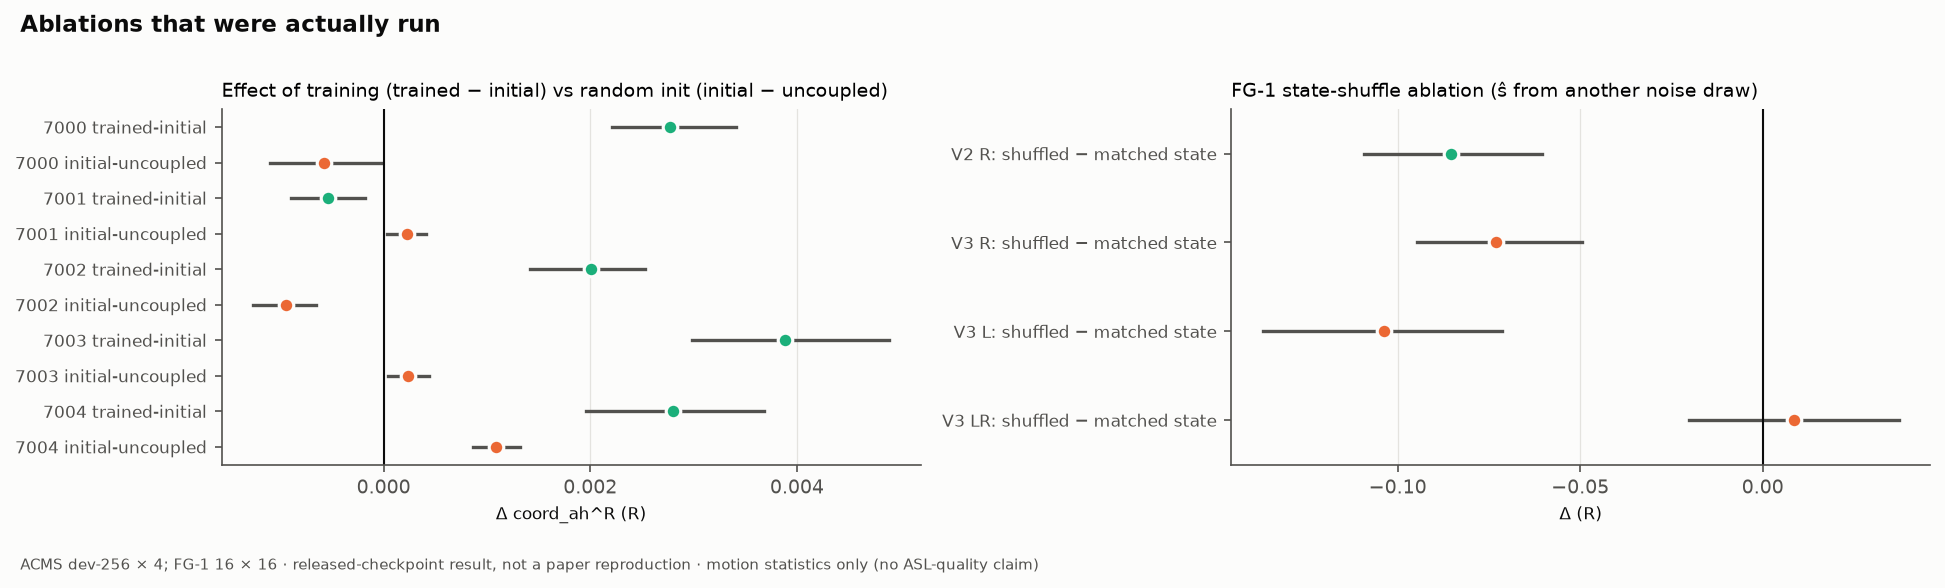
\includegraphics[width=\textwidth]{figures/f12_ablations.png}\caption{Ablations that were actually run.}\end{figure*}
\begin{table}[t]\centering\caption{Measured computational cost (single RTX A4000 16 GB)}\footnotesize\begin{tabular}{llll}\toprule \textbf{Experiment} & \textbf{Wall-clock (min)} & \textbf{Peak GPU reserved (GiB)} & \textbf{Trainable params} \\ \midrule Stage 4 E2e (fixed M-C, 16 conditions) & 28.8 & not logged & 0 \\ Stage 4 E2c (ii) (per-clip M-C, 32 clips) & 26.9 & 8.70 & $\approx$9,060/clip \\ ACMS train run 7000 & 4.7 & 10.72 & 433 \\ ACMS eval run 7000 (R+J) & 27.3 & 10.78 & 0 \\ ACMS train run 7001 & 4.7 & 10.75 & 433 \\ ACMS eval run 7001 (R+J) & 28.2 & 10.78 & 0 \\ ACMS train run 7002 & 4.7 & 10.82 & 433 \\ ACMS eval run 7002 (R+J) & 25.9 & 10.78 & 0 \\ ACMS train run 7003 & 4.5 & 10.77 & 433 \\ ACMS eval run 7003 (R+J) & 25.9 & 10.78 & 0 \\ ACMS train run 7004 & 4.6 & 10.69 & 433 \\ ACMS eval run 7004 (R+J) & 25.9 & 10.78 & 0 \\ FG-1 prep & 2.8 & 10.52 & 0 \\ FG-1 V1 & 53.3 & 10.52 & 9060 \\ FG-1 V2 & 53.0 & 10.52 & 433 \\ FG-1 V3 & 103.4 & 10.52 & 866 \\ optg\_s7000 & 4.3 & 10.72 & 0 \\ optg\_s7001 & 4.3 & 10.75 & 0 \\ optg\_s7002 & 4.3 & 10.82 & 0 \\ optg\_s7003 & 4.3 & 10.77 & 0 \\ optg\_s7004 & 4.3 & 10.69 & 0 \\ optc\_s7000\_u025 & 8.1 & 10.78 & 0 \\ optc\_s7000\_u050 & 8.1 & 10.78 & 0 \\ optc\_s7000\_u075 & 8.1 & 10.78 & 0 \\ optc\_s7000\_u100 & 8.1 & 10.78 & 0 \\ optc\_s7001\_u025 & 8.1 & 10.78 & 0 \\ optc\_s7001\_u050 & 8.1 & 10.78 & 0 \\ optc\_s7001\_u075 & 8.1 & 10.78 & 0 \\ optc\_s7001\_u100 & 8.1 & 10.78 & 0 \\ optc\_s7002\_u025 & 8.1 & 10.78 & 0 \\ optc\_s7002\_u050 & 8.1 & 10.78 & 0 \\ optc\_s7002\_u075 & 8.1 & 10.78 & 0 \\ optc\_s7002\_u100 & 8.1 & 10.78 & 0 \\ optc\_s7003\_u025 & 8.1 & 10.78 & 0 \\ optc\_s7003\_u050 & 8.2 & 10.78 & 0 \\ optc\_s7003\_u075 & 8.2 & 10.78 & 0 \\ optc\_s7003\_u100 & 8.2 & 10.78 & 0 \\ optc\_s7004\_u025 & 8.2 & 10.78 & 0 \\ optc\_s7004\_u050 & 8.2 & 10.78 & 0 \\ optc\_s7004\_u075 & 8.2 & 10.78 & 0 \\ optc\_s7004\_u100 & 8.1 & 10.78 & 0 \\ \bottomrule\end{tabular}\end{table}
\begin{figure*}[t]\centering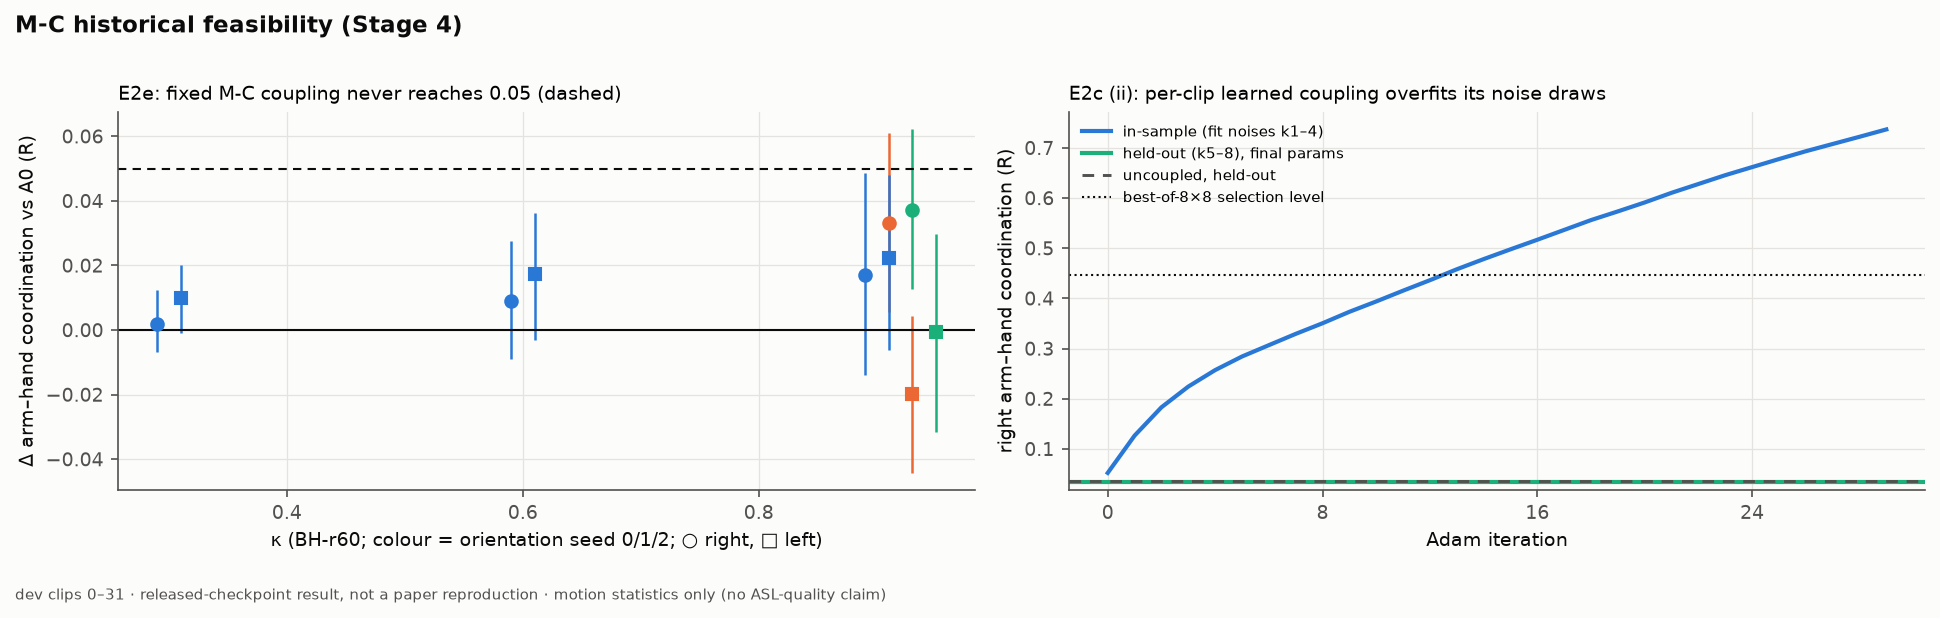
\includegraphics[width=\textwidth]{figures/f07_mc_history.png}\caption{Historical M-C feasibility (Stage 4): fixed coupling (E2e) and per-clip learned coupling (E2c (ii)).}\end{figure*}
\section{Consolidated results}
\begin{table*}[t]\centering\caption{All executed experiments (released-checkpoint results; space R)}\footnotesize\begin{tabular}{lllll}\toprule \textbf{Experiment} & \textbf{Unit / n} & \textbf{Primary statistic (R)} & \textbf{Estimate [95\% CI]} & \textbf{Outcome} \\ \midrule Stage 4 E2e fixed M-C coupling & 16 conditions, 32 dev clips & $\Delta$ arm--hand (T3) & R 0.017, L 0.022 (CIs incl. 0) & FM13 stop (negative) \\ Stage 4 E2c (ii) per-clip M-C & 32 dev clips & held-out gain & -0.003 [-0.017, +0.012] & negative (FM4) \\ Stage 5 ACMS, run 7000 & dev-256 $\times$ 4 & $\Delta$ trained -- uncoupled & +0.0022 [+0.0014, +0.0031] & positive, negligible \\ ACMS multi-seed (7001--7004) & 4 runs & pooled $\Delta$ (t) & +0.0022 [-0.0013, +0.0056] & seed-sensitive \\ ACMS all five runs (secondary) & 5 runs & pooled $\Delta$ (t) & +0.0022 [-0.0001, +0.0045] & seed-sensitive \\ OPT-G train-like generalisation & 4 new runs & pooled $\Delta$ on own TRAIN clips & +0.0019 [-0.0015, +0.0053] & monitoring \\ FG-1 V1 & 16 TRAIN clips $\times$ 16 & held-out $\Delta$ vs V0 & +0.0034 [-0.0121, +0.0166] & negative \\ FG-1 V2 & 16 TRAIN clips $\times$ 16 & held-out $\Delta$ vs V0 & +0.1016 [+0.0753, +0.1288] & inconclusive \\ FG-1 V3 & 16 TRAIN clips $\times$ 16 & held-out $\Delta$ vs V0 & +0.0893 [+0.0703, +0.1091] & positive \\ \bottomrule\end{tabular}\end{table*}
\begin{table*}[t]\centering\caption{Metric coverage: measured (registered outputs), derived (post-hoc, from saved outputs), unavailable, not used}\footnotesize\begin{tabular}{lll}\toprule \textbf{Metric} & \textbf{Status} & \textbf{Source / reason} \\ \midrule Arm--hand coordination coord\_ah\textasciicircum{}R (right; primary), L, L--R, dominance (R) & measured & registered evaluation, dev-256 $\times$ 4 \\ J-space coordination (SMPL-X) & measured (descriptive) & not gating; \textasciitilde{}1--2\% skinning leakage \\ Preservation ratios, extremes, activity, undefined fraction, KL/frame & measured & registered checks \\ Training return R per episode (logged) & measured & episodes.json; reproduced exactly by the registered reward \\ FG-1 held-out $\Delta$, in-sample $\Delta$, generalisation gap, state shuffle & measured & FG-1 gate outputs \\ Runtime, peak GPU memory & measured & runner logs \\ Evaluation return R per sample (trained / initial / uncoupled) & derived (post-hoc) & registered reward applied to eval\_samples.json \\ Paired return difference, cumulative reward difference, paired win fraction & derived (post-hoc) & baseline-relative; not regret \\ Training return progression and twin-relative cumulative difference & derived (post-hoc) & episodes.json \\ Regret (optimal minus achieved return) & unavailable & no optimal-policy reference in the design \\ Task success rate & unavailable & no episodic task or success criterion exists \\ FID / diversity / multimodality & unavailable & no validated ASL feature extractor \\ PPO / GRPO / SAC comparison & unavailable & never run; no comparative claim made \\ DTW-JPE / MPJPE vs. reference as success measure & not used & favours collapse in GF (static mean beats samples; M5--M6) \\ BLEU / back-translation & not used & within-text uncorrelated with pose error; hackable by selection (R6) \\ Perceptual naturalness, intelligibility, ASL quality & out of scope & human evaluation removed (rev. 4.0) \\ How2Sign test split & never opened & only registered TRAIN and DEV used \\ \bottomrule\end{tabular}\end{table*}
The project's slide deck from earlier stages was not present in the workspace, so direct deck-to-deck coverage verification was \textbf{unavailable}; metric coverage was checked against the written coverage plan (\texttt{PPT\_METRIC\_COVERAGE.md}) instead.

\section{Post-hoc analysis: episodic return and baseline-relative statistics (not pre-registered)}
\textbf{This section is post-hoc and was not pre-registered.} It re-expresses saved outputs in reinforcement-learning terms. It ran on CPU only, generated no samples, changed no file outside \texttt{experiments/stage6\_final/posthoc\_return/}, and changes no registered threshold, verdict or category. The primary pre-registered statistic remains coord\_ah\textasciicircum{}R, reported in the multi-seed results section.

\subsection{Definitions}
Each episode is a single decision (one noise draw $\rightarrow$ one sample), so the episodic return equals the registered reward, recomputed with the unchanged implementation (\texttt{experiments/stage5/rewards.py}, \texttt{episode\_reward}):

\begin{center}R = r\_ah -- $\Sigma$\_k $\lambda$\_k c\_k,   r\_ah = --|coord\_ah\textasciicircum{}R -- $\tau$|,   $\tau$ = 0.4514 (frozen);   undefined coord $\rightarrow$ r\_ah = --(1 + $\tau$)\end{center}
$\lambda$\_k = 0 in every run at every update, so R = r\_ah; the constraint terms c\_k use each sample's uncoupled twin (same clip and noise index), exactly as in training. Evaluation: dev-256, 256 clips $\times$ 4 noise draws $\times$ 3 conditions per run (1024 samples per condition); 0 undefined coordinations across all runs and conditions. Paired difference for clip i and noise k:

\begin{center}d\_ik = R(trained, i, k) -- R(uncoupled, i, k);   CRD = $\Sigma$\_ik d\_ik;   win = mean\_ik 1[d\_ik > 0]\end{center}
Within a run, CIs are clip bootstraps over clip means of d (B = 2000, seed 0); across runs, t-intervals with runs as the unit, as in the registered analysis. Clip win fraction = share of clips whose mean d is positive. Training statistics use the 500 logged episodes per run (125 updates $\times$ 4 TRAIN episodes); the twin-relative difference is R(controlled) -- R(uncoupled twin) on the same training noise. Every logged training return was reproduced exactly by the registered reward (maximum absolute error 0).

\subsection{Held-out evaluation return}
\begin{table*}[t]\centering\caption{Post-hoc evaluation return on dev-256 $\times$ 4 (update 125). Return = --|coord\_ah\textasciicircum{}R -- 0.4514|; higher is better; CRD = cumulative reward difference over 1024 paired samples. Not regret.}\footnotesize\begin{tabular}{llllllll}\toprule \textbf{Run} & \textbf{Return trained} & \textbf{Return uncoupled} & \textbf{$\Delta$ trained -- uncoupled [95\% CI]} & \textbf{$\Delta$ trained -- initial} & \textbf{Win (samples)} & \textbf{Win (clips)} & \textbf{CRD (1024)} \\ \midrule 7000 & -0.4322 & -0.4344 & +0.0023 [+0.0015, +0.0032] & +0.0028 [+0.0022, +0.0034] & 0.588 & 0.613 & +2.323 \\ 7001 & -0.4347 & -0.4344 & -0.0003 [-0.0007, +0.0002] & -0.0005 [-0.0009, -0.0002] & 0.473 & 0.477 & -0.285 \\ 7002 & -0.4334 & -0.4344 & +0.0011 [+0.0005, +0.0016] & +0.0021 [+0.0015, +0.0026] & 0.547 & 0.609 & +1.117 \\ 7003 & -0.4303 & -0.4344 & +0.0042 [+0.0032, +0.0052] & +0.0039 [+0.0030, +0.0048] & 0.667 & 0.781 & +4.256 \\ 7004 & -0.4306 & -0.4344 & +0.0039 [+0.0029, +0.0049] & +0.0028 [+0.0020, +0.0037] & 0.605 & 0.695 & +3.970 \\ Pooled 4 new (t) & -0.4322 [-0.4357, -0.4288] & -0.4344 [-0.4344, -0.4344] & +0.0022 [-0.0012, +0.0057] & +0.0021 [-0.0009, +0.0050] & +0.573 [+0.441, +0.705] & +0.641 [+0.434, +0.847] & +2.26 [-1.26, +5.79] \\ Pooled all 5 (t) & -0.4322 [-0.4346, -0.4299] & -0.4344 [-0.4344, -0.4344] & +0.0022 [-0.0001, +0.0045] & +0.0022 [+0.0002, +0.0042] & +0.576 [+0.486, +0.666] & +0.635 [+0.495, +0.776] & +2.28 [-0.10, +4.66] \\ \bottomrule\end{tabular}\end{table*}
Uncoupled return is identical in every run (-0.4344, per-sample SD 0.161), as the uncoupled samples are bitwise identical. The pooled paired return gain (4 new runs) is +0.0022 [-0.0012, +0.0057], which matches the registered coordination result because 98.4\% or more of samples in every run and condition lie below $\tau$, where return and coordination move together. The paired win fraction is +0.573 [+0.441, +0.705] over samples and +0.641 [+0.434, +0.847] over clips; both intervals include 0.5. The five-run trained -- initial difference +0.0022 [+0.0002, +0.0042] has a lower bound above zero, but this is a post-hoc secondary contrast and does not alter the registered seed-sensitive category.

\subsection{Training return}
\begin{table*}[t]\centering\caption{Post-hoc training return on each run's TRAIN clips (logged, 500 episodes). Training return is not held-out return: clips are sampled from TRAIN and differ between updates.}\footnotesize\begin{tabular}{lllllllll}\toprule \textbf{Run} & \textbf{Episodes} & \textbf{Mean R} & \textbf{SD R} & \textbf{SD of update means} & \textbf{First 25 updates} & \textbf{Last 25 updates} & \textbf{Twin-relative CRD} & \textbf{Twin win} \\ \midrule 7000 & 500 & -0.4275 & 0.1778 & 0.0905 & -0.4202 & -0.4381 & +0.012 & 0.534 \\ 7001 & 500 & -0.4206 & 0.1701 & 0.0887 & -0.4180 & -0.4027 & +0.157 & 0.522 \\ 7002 & 500 & -0.4269 & 0.1745 & 0.0808 & -0.4205 & -0.4143 & +0.035 & 0.490 \\ 7003 & 500 & -0.4219 & 0.1716 & 0.0814 & -0.4030 & -0.4220 & +0.907 & 0.622 \\ 7004 & 500 & -0.4110 & 0.1797 & 0.0883 & -0.4473 & -0.3622 & +1.187 & 0.586 \\ Pooled 4 new (t) &  & -0.4201 [-0.4307, -0.4095] &  &  &  & last -- first +0.0219 [-0.0490, +0.0927] & +0.571 [-0.325, +1.468] &  \\ \bottomrule\end{tabular}\end{table*}
Training return is dominated by clip-to-clip variation (episode SD $\approx$ 0.17; SD of 4-episode update means $\approx$ 0.08--0.09), so changes between the first and last 25 updates (pooled +0.0219 [-0.0490, +0.0927]) mostly reflect which clips were drawn. The twin-relative difference removes clip and noise effects: its cumulative sum over 500 episodes grows clearly only in runs 7003 and 7004, the two runs with the largest held-out gains.

\begin{figure*}[t]\centering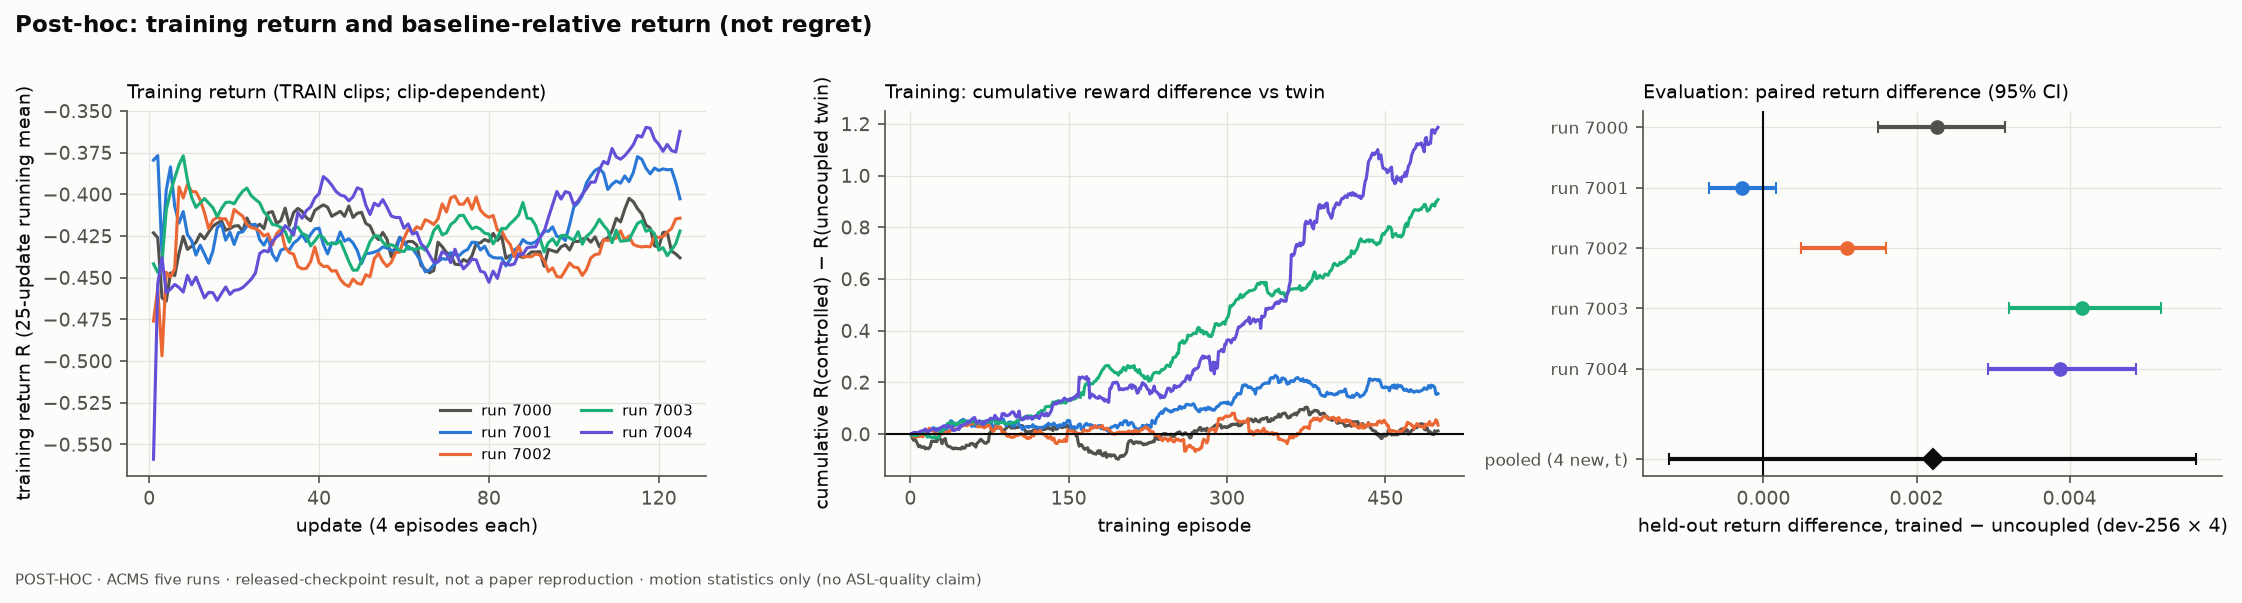
\includegraphics[width=\textwidth]{figures/f13_posthoc_return.png}\caption{Post-hoc: training return (25-update running mean), training cumulative reward difference vs the uncoupled twin, and held-out paired return difference per run. Not regret.}\end{figure*}
\subsection{Regret}
\textbf{Conventional regret cannot be calculated.} The saved design has no optimal-policy reference: (i) the reward supremum 0 (coord\_ah\textasciicircum{}R = tau exactly) is a property of the reward function, not the value of any known or attainable policy; (ii) the best-of-8x8 (0.408) and FG-1 best-of-16 contexts are selection oracles over noise draws that use the outcome, not policies; (iii) per-clip FG-1 fits are a different estimator, clip set and noise set. No optimal reward, success criterion or regret bound is defined here. The statistics in this analysis are baseline-relative (trained minus uncoupled) and must not be read as regret.

\subsection{Limitations of the post-hoc analysis}
\begin{itemize}\item Not pre-registered; reported for completeness and interpretability only.\item Return is a monotone transform of the primary statistic below $\tau$, so it is not independent evidence.\item Win fractions ignore effect size; a 0.6 win fraction here coexists with a mean gain of about 0.002.\item Cumulative reward differences scale with the number of samples (1024 in evaluation, 500 in training) and are not comparable across the two.\item Training statistics are on TRAIN clips under a changing policy; they are not generalisation estimates.\end{itemize}
\section{Discussion}
Three controller families now have measured held-out evidence on the frozen SignSparK sampler. Fixed M-C coupling (E2e) failed its registered gate. Per-clip learned M-C coupling (E2c (ii)) fits its own noise draws to an in-sample coordination of 0.74 (above the 0.45 reference level) yet transfers nothing to fresh noise. Amortised ACMS gives a positive \emph{direction} in three of four new runs but a magnitude about 1/23 of the relevance threshold, with high across-seed heterogeneity. FG-1 places all families on identical clips and noises. Fitted per clip on that clip's own noise draws, the same 433-parameter ACMS family (V2) raises held-out right arm--hand coordination by +0.1016 [+0.0753, +0.1288] on fresh noise, but its articulation ratio (1.102) exceeds the registered 1.10 bound, so its outcome is inconclusive; the bilateral variant (V3) gives +0.0893 [+0.0703, +0.1091] with preservation passing and is positive on the primary statistic. Learned M-C coupling (V1) again fits strongly in sample (+0.494 [+0.442, +0.545]) and transfers almost nothing (+0.0034 [-0.0121, +0.0166]).

The contrast between FG-1 and the multi-seed result locates the bottleneck. A state-conditioned mean shift within a KL budget of about 0.1 nats/frame \textbf{can} move coordination by more than 0.05 on fresh noise when it is fitted to one clip, and the state-shuffle ablation shows that the gain depends on conditioning on the matching arm signal. The amortised policy, one 433-parameter controller shared across all training clips and trained with REINFORCE, captures only a few per cent of that. A plausible interpretation, consistent with Stage 4 Theorem 3, is that the useful arm-to-hand mapping in noise space is clip-specific, so a single shared controller averages it away. This is an interpretation, not a tested claim: FG-1 used pathwise gradients rather than RL, so it does not separate the effect of amortisation from that of the gradient estimator.

The results do \textbf{not} show that RL cannot improve SignSparK in general; they apply to noise-space control of a frozen checkpoint with the registered motion-statistic reward. Fine-tuning, architectural coupling of the hand generators, and perceptual or semantic objectives were outside scope.

\section{Limitations and threats to validity}
\begin{itemize}\item Four new training runs give a wide t-interval (t-critical 3.18); the seed-sensitive category reflects both heterogeneity and low power.\item Coordination in R is a motion statistic validated only automatically (V-R1--V-R4); perceptual validity is out of scope.\item J statistics include SMPL-X skinning leakage (\textasciitilde{}1--2\% of hand signal); used descriptively only.\item FG-1 uses 16 TRAIN clips and one fit per clip (no seed replication); per-clip fitting with pathwise gradients tests controllability, not an amortised or deployable RL policy, and needs the clip in advance.\item V2 misses the articulation-ratio bound narrowly; the bound was applied as registered and not revisited.\item The checkpoint's pretraining split usage is undocumented (possible How2Sign leakage), irrelevant to relative comparisons but relevant to absolute levels.\item cuDNN non-determinism is permitted (TF32 off for matmul); repeated runs may differ in low-order bits.\end{itemize}
\section{Conclusion}
On the evidence obtained, amortised noise-space RL on the frozen SignSparK checkpoint does not produce a practically relevant improvement in arm--hand coordination. The only positive pre-registered training result (ACMS run 7000) replicates in direction in three of four new seeds, but the pooled effect +0.0022 [-0.0013, +0.0056] is \textbf{seed-sensitive} and about 23 times below the registered threshold. Preservation holds throughout. In the FG-1 fresh-noise gate: learned M-C negative (held-out $\Delta$ +0.0034); per-clip ACMS inconclusive (held-out $\Delta$ +0.1016); bilateral SC-MC positive (held-out $\Delta$ +0.0893). Per-clip, state-conditioned noise control is therefore feasible on fresh noise, but turning it into a single policy that works across clips was not achieved. The project is closed on this evidence.

\section*{Reproducibility statement}
All code, configurations, seeds, commands, runtimes, GPU memory and SHA-256 hashes are listed in \texttt{research/final/EXPERIMENT\_MANIFEST.json}. Environment: Windows 11, Python 3.12, torch 2.10.0+cu128, RTX A4000 16 GB. Released SignSparK checkpoints (body bf95bb02\ldots{}, hand 5bb8e407\ldots{}) were verified unchanged after all runs.

\begin{thebibliography}{9}
\bibitem{r1} J. He et al., "SignSparK: Efficient multilingual sign language production via sparse keyframe learning," ECCV 2026 (released code github.com/JianHe0628/SignSparK and checkpoints HF LionelLow/SignSparK).
\bibitem{r2} A. Duarte et al., "How2Sign: A large-scale multimodal dataset for continuous American Sign Language," CVPR 2021.
\bibitem{r3} R. J. Williams, "Simple statistical gradient-following algorithms for connectionist reinforcement learning," Machine Learning, 1992.
\bibitem{r4} W. Kool, H. van Hoof, M. Welling, "Buy 4 REINFORCE samples, get a baseline for free!," ICLR DeepRL Meets Structured Prediction Workshop, 2019.
\bibitem{r5} E. Altman, Constrained Markov Decision Processes, Chapman \& Hall/CRC, 1999.
\bibitem{r6} J. Liu et al., "Flow-GRPO: Training flow matching models via online RL," arXiv 2505.05470, 2025.
\bibitem{r7} K. Clark et al., "Directly fine-tuning diffusion models on differentiable rewards (DRaFT)," ICLR 2024.
\bibitem{r8} L. Eyring et al., "Noise hypernetworks: Amortizing test-time compute in diffusion models," NeurIPS 2025 (arXiv 2508.09968).
\bibitem{r9} G. Pavlakos et al., "Expressive body capture: 3D hands, face, and body from a single image (SMPL-X)," CVPR 2019.
\bibitem{r10} R. DerSimonian, N. Laird, "Meta-analysis in clinical trials," Controlled Clinical Trials, 1986.
\bibitem{r11} B. Efron, R. Tibshirani, An Introduction to the Bootstrap, Chapman \& Hall, 1993.
\bibitem{r12} X. Liu, C. Gong, Q. Liu, "Flow straight and fast: Learning to generate and transfer data with rectified flow," ICLR 2023.
\end{thebibliography}\end{document}